\newpage
\thispagestyle{empty}

\noindent
Ted Sundstrom \\
Professor Emeritus, Grand Valley State University \\
Allendale, MI\\
%mathreasoning@gmail.com


%\quarter
%\newpar
%\eighth
\noindent
\emph{Mathematical Reasoning: Writing and Proof}

\noindent
Copyright \copyright \, \the\year, 2013 ~by Ted Sundstrom

\noindent
See page~(\pageref{C:versions}) for a comparison of Version 2.1 and Version 3.

%\newpar
\noindent
Previous versions of this book were published by Pearson Education, Inc.

%\section*{Changes Made in Version 1.1}
%There are no changes in content between version 1.0 of this book and version 1.1.  The only changes are  the addition of the \emph{Note to Students} immediately following the Table of Contents, and the Creative Commons License has been changed to the Creative Commons Attribution-NonCommercial-ShareAlike
%3.0 Unported License.
%\section*{Changes Made in Version 2.0}
%There are no changes in content between Version 1.1 of this book and Version 2.0.  The only change is  that Appendix~\ref{C:answers}, Answers and Hints for Selected Exercises, now contains solutions and hints for more exercises.  Those exercises with an answer or a hint in the appendix are preceded by a star $\left( ^\star \right)$.
%\section*{Changes Made in Version 2.1}
%\section*{Changes Made in Version 3}
%The main change in Version 3 is that the preview activities have been renamed to beginning activities.  This was done to emphasize that these activities are meant to be completed before starting the rest of the section.  
%In addition, two beginning activities have been added to Section 1.1.  (There are no preview activities in Section 1.1 of Version 2.1.)


%The only change is  that Appendix~\ref{C:answers}, Answers and Hints for Selected Exercises, now contains solutions and hints for more exercises.  Those exercises with an answer or a hint in the appendix are preceded by a star $\left( ^\star \right)$.

\section*{License}
%This work is licensed under the Creative Commons Attribution-NonCommercial-No Derivative Works
%3.0 Unported License. The graphic
%\begin{center}
%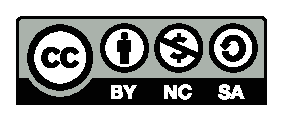
\includegraphics{CClicense.eps}
%%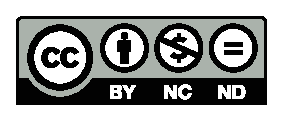
\includegraphics{CC-by-nc-nd.eps}
%\end{center}
%that appears throughout the text shows that the work is licensed with the Creative Commons, that
%the work may be used for free by any party so long as attribution is given to the author.  In addition, this work may not be altered or transformed and no party may
%sell this work for profit. Full details may be found by visiting
%\begin{center}
%http://creativecommons.org/licenses/by-nc-nd/3.0/
%\end{center}
%or sending a letter to Creative Commons, 444 Castro Street, Suite 900, Mountain View, California,
%94041, USA.
This work is licensed under the Creative Commons Attribution-NonCommercial-ShareAlike
3.0 Unported License. The graphic
\begin{center}
\scalebox{0.75}{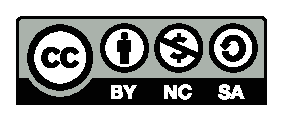
\includegraphics{CClicense.eps}}
\end{center}
that appears throughout the text shows that the work is licensed with the Creative Commons, that
the work may be used for free by any party so long as attribution is given to the author(s), that the
work and its derivatives are used in the spirit of ``share and share alike,'' and that no party other than the author(s) may
sell this work or any of its derivatives for profit. Full details may be found by visiting
%\begin{center}
%http://creativecommons.org/licenses/by-nc-sa/3.0/
%%http://creativecommons.org/licenses/by-nc-nd/3.0/
%\end{center}

\begin{center}
%\href{http://creativecommons.org/licenses/by-nc-sa/3.0/}
\url{http://creativecommons.org/licenses/by-nc-sa/3.0/}
%http://creativecommons.org/licenses/by-nc-nd/3.0/
\end{center}
or sending a letter to Creative Commons, 444 Castro Street, Suite 900, Mountain View, California,
94041, USA.

%\newpar
%\textbf{Cover Photograph}: The Little Mac Bridge on the campus of Grand Valley State University in Allendale, Michigan.
\newpage
\thispagestyle{empty}
$ $
\endinput

\endinput
